\documentclass[../../main.tex]{subfiles}
\graphicspath{{\subfix{../../diagrams/}}}
\usepackage{lipsum}  
\usepackage{float}

\begin{document}
\begin{figure}[h!]
\caption{Shop module class diagram.}
\vspace{10mm}
\centering
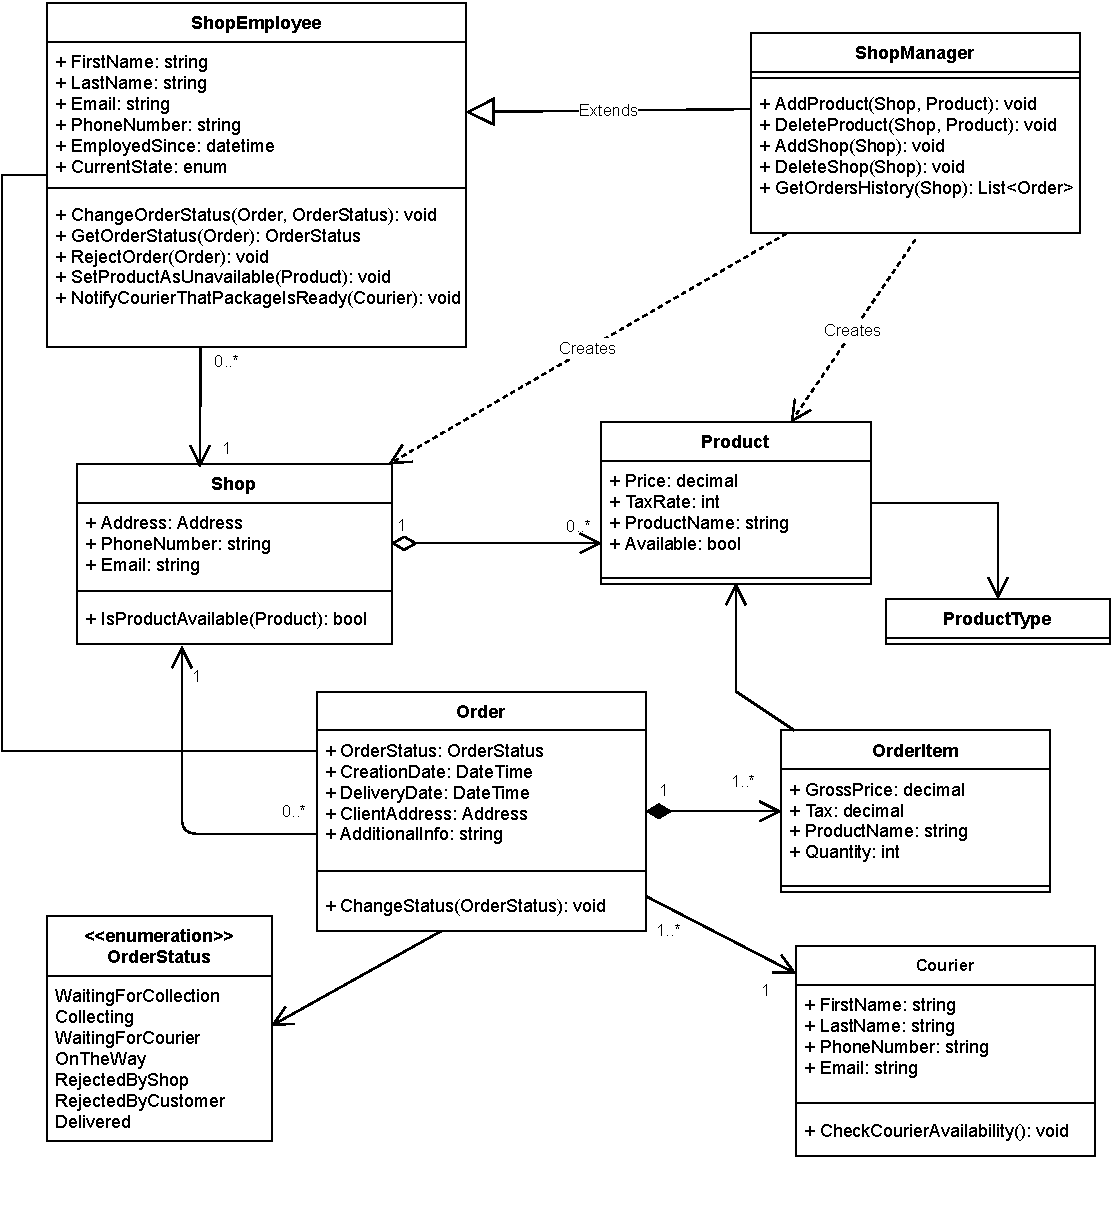
\includegraphics[width=1\textwidth]
{class-diagrams/shop-class-diagram.pdf}
\end{figure}
\newpage

\subsubsection{Shop}

Shop object is an individual shop facility of a given retail chain (like Carrefour for example). Each Shop object has many ShopEmployees and at least one ShopManager, who are main actors in this module. Furthermore, each Shop has an offer of available products (the subset of global product offer, which is also handled by the shop module). In addition to this, each shop object contains orders, which were handled or are being processed by a given Shop. 

\subsubsection{Order}

After the order is created in client module, it goes to shop module, where it is being prepared and packed. Each order consists of many OrderItems, which are basically Products from shop offer, but with Quantity and GrossPrice (including tax) calculated. Orders are assigned to courier, who is responsible for delivering the order to customer. At any time, ShopEmployee, who is preparing the order can contact with the corresponding courier. Moreover, each order has OrderStatus, which are listed in the diagram. Status can be modified by ShopEmployee during orders processing. 

Available order statuses:
\begin{itemize}
  \item WaitingForCollection -- order is waiting to be processed by one of the ShopEmployee
  \item Collecting -- order is being prepared by the ShopEmployee
  \item WaitingForCourier -- order is prepared; it is waiting for the courier
  \item OnTheWay -- order is being delivered by the courier
  \item RejectedByShop -- order is reject by the shop
  \item RejectedByClient -- order is reject by the client 
  \item Delivered -- order is delivered to client
\end{itemize}

\subsubsection{ShopEmployee}

ShopEmployee can preform basic actions regarding Order processing like changing OrderStatus or notifying courier, that the package is ready to pick up. Furthermore, ShopEmployee can also set product as unavailable in the shop facility, where he/she works.  
 
\subsubsection{ShopManager}

ShopManager extends ShopEmployee and has additional actions regarding product offer and shop facility grid management. ShopManager can add/remove product from the global product offer and add/remove shop from the facility grid. In addition, ShopManager can get reports of shop efficiency (number of prepared orders in a given month) and inspect orders history.

\subsubsection{Product}

In the shop module workers can also manage the list of products available for the customers. There are three entities, which relate to products:
\begin{itemize}
  \item ProductType -- globally available product in a given retail chain (like 1L bottle of Coca-Cola)
  \item Product -- product in a given shop facility (it is very similar to ProductType, but it only refers to a single shop facility). It contains Available field, which indicates, whether the product is available in a shop facility. For example: Coca-Cola is available in Carrefour in Warsaw, ul. Marszałkowska 22, but it is not available in Carrefour in Kraków, ul. Długa 11)
  \item OrderItem -- product in the order, it has quantity and GrossPrice properties. For example: two bottles of 1L Coca-Cola ordered by Jan Kowalski from Carrefour.
\end{itemize}

\end{document}